\documentclass{article}

\usepackage{graphicx}
\usepackage{amsmath}

\begin{document}

In this blog post, I'd like to quickly go over some very basic techniques in molecular biology. I'm
going to stick strictly to the big ideas; these ideas should be enough to get you reading papers,
but certainly not enough to be performing these procedures in a lab.

\section*{Plasmid transformation}
Plasmid transformation is a mechanism by which we can introduce genes of interest into bacterial
cells. In order to do this, we isolate another plasmid, insert the gene we want, and then put the
plasmid back into the bacterial cells.

We can isolate the plasmid via various biochemical means, and plasmids are small enough such that we
can isolate \emph{whole} plasmids. (We have difficult isolating whole pieces of longer DNA, which
tends to break up into fragments.) Once we have isolated the plasmid, we can apply restriction
enzymes (such as EcoRI) for the specific sequences that we want to the plasmid and the gene of
interest. The restriction enzymes cleave the plasmid and our gene at cut sites; often, this leaves
stick ends (ends of DNA with a single-stranded strand between two and four bases long). These sticky
ends readily bond back together with other matching DNA pieces; in this manner, we can join the gene
of interest into our plasmid or cut other pieces out of the plasmid. After adding the restriction
enzyme, we add DNA ligase to ligate the plasmid back together (to reform the covalent bonds that
hold the DNA together).

Once we have our ligated plasmid, we would like to insert it into bacterial cells. Some bacteria are
naturally competent, and will simply accept plasmids from their environment. However, many other
bacteria (such as \emph{E. Coli}), are not naturally competent, and we have to induce competence in
order to get them to accept the plasmid. There are electrical methods to induce competence, which
apply a field and essentially break the bacteria open in order to accept the plasmid; although most
of the bacteria die, some survive and form colonies. There are also chemical methods to induce
competence, such as adding calcium chloride to \emph{E. Coli}, but their mechanism of action is more
complicated.

Finally, once we have inserted our plasmid into bacterial cells, we can grow them back into
colonies. If we need to, we can apply selection for recombinant plasmids, which is discussed later
in this technique primer.

\section*{Restriction digestion}
A restriction enzyme is a protein which cleaves DNA at specific sequences. The resulting break in
the DNA can be used to insert other pieces of DNA into that location, after which DNA ligase can be
used to join the DNA back together.

The sequences at which restriction enzymes operate are usually the same from 5' to 3' (they are DNA
palindromes). The reason for this is that restriction enzymes are usually dimers where each monomer
in the dimer operates on a single strand. If the sequence is palindromic, then both monomers will
bind to the same location on the strand.

Restriction enzymes are specific to sequence and also the type of cut they make. They can create
blunt ends in the cut (where the cut is in the middle of the sequence), resulting in entirely double
stranded DNA, all the way up until the break. They can also create what is known as ``sticky ends''.
A sticky end is a piece of DNA which at end of one strand has a small single-stranded portion, which
is created because the restriction enzyme cuts the sequence off-center. This single-stranded portion
can be between two and four bases long, and matches the single stranded portion on the other half of
the break. Since they match, having them join together is energetically favorable (since it forms
hydrogen bonds between the single-stranded portions), so it is more likely to happen; this is why
these are referred to as ``sticky'' ends.

When the DNA joins back together with hydrogen bonds, there is no reason why it should join back in
the exact same configuration as before. Because of this, we can cleave DNA and insert other pieces
of DNA (with matching sticky ends) into that region. After that, we can use DNA ligase to covalently
bond the pieces of DNA back together.

\section*{Electrophoresis}
Electrophoresis is a process by which we can separate DNA fragments based on their molecular weight,
and visually inspect what different sizes exist, as well as measure the sizes of the DNA fragments.

In order to do DNA electrophoresis, we begin by preparing the DNA fragments we're interested in. In
some cases, these come from restriction enzymes being applied to larger fragments, but that is in no
way required or a characteristic of electrophoresis. We then create an agar gel which is put into a
plate; this plate must have two electrodes on the sides.

Once the plate is prepared, we place DNA in wells in the agar gel on the side of the negative
electrode. An electric field is applied between the two electrodes, and due to the negative charge
on the phosphates, the DNA migrates towards the positive electrode. The electric field is held on
for a while and then turned off. Smaller fragments will encounter less resistance from the gel, and
will thus travel faster, while larger fragments which have a harder time getting through pores in
the gel will travel slower. The distance traveled is related more or less logarithmically to the
size of the molecule, because smaller pieces experience exponentially less resistance than larger
ones.

Note that if you have fragments of similar size, it may be impossible to discriminate between them,
because they will be placed next to each other. However, you can increase the time period over which
the gel is run to reduce this.

In order to visualize the results, we add ethidium to the gel (or afterwards). Ethidium is a dye
which binds to the DNA and sits inside the DNA helix. As the DNA migrates, it collects ethidium and
thus has it in much greater concentrations than the surrounding gel. Ethidium glows under
ultraviolet light, thus allowing us to see where the bands of DNA are.

For large pieces of DNA, gel electrophoresis may be ineffective, because the large pieces all will
move at the same speed. In order to get around this, we can use pulsed electrophoresis. In this
case, there are more electrodes on the edges, and the field points always towards the positive end
of the plate but diagonally up or down; the field is pulsed in these two directions. The directions
average out to a straight line, but due to the fact that the field changes rapidly, the DNA must
reorient itself. Larger fragments take longer to reorient themselves, and thus this technique may be
used to separate large DNA fragments that would otherwise travel together.

Given DNA marker fragments of known size, we can use electrophoresis to compute the size of the
fragments. We can also use this technique for the purpose of sequencing DNA (Sanger sequencing).
\section*{Ligation}
DNA Ligase is an enzyme which is responsible for covalently joining together pieces of DNA or
nucleotides. In \emph{in vivo} DNA replication, ligase fills in the nicks (un-bound DNA pieces) left
after lagging strand replication. (Recall that the RNA primers are degraded after which DNA
polymerase adds bases to fill in the gap left by the primer, but it cannot covalently join the new
bases to the bases that were there after the primer; this is what is done by DNA ligase.) 

We can use DNA ligase in combination with restriction enzymes to cut up DNA and then put it back
together. For instance, we can use this to create recombinant plasmids.

Ligase works better with sticky ends left by restriction enzymes, but will work fine with blunt ends
as well, although higher concentrations will be required.

\section*{Selection for recombinant plasmids}
When creating recombinant plasmids and transforming bacteria with them, we may end up with bacteria
with both the recombinant and original version of the plasmid. However, we may want to select only
for the recombinant plasmid. In some cases, this is natural, and we can do so by just selecting for
the property that the recombinant plasmid gives us.

Often, however, we will need to use more advanced techniques to select for the recombinant plasmid.
In order to do this we can add in a second gene of interest, which we can then use to select for our
plasmid. For instance, we can add a gene for a specific antibiotic resistance; then, we can grow our
transformed bacteria on that antibiotic. The bacteria that have the original plasmid will die, while
our transformed bacterial cells (which have that extra gene) will be selected for. 

We can also do similar things with other genes. For instance, we could insert a fluorescent gene
such as GFP.\@ Once the colonies grow, we can examine them visually and select the ones that exhibit 
the fluorescence we want. This way, we can select only the colonies that have our plasmid.

\section*{Sanger Sequencing}

Sanger Sequencing is a technique for obtaining the sequence of bases (As, Cs, Gs, and Ts) that
compose some piece of DNA.\@ It is one of the first methods developed, and, with minor improvements,
is still in use today. Although it has much lower throughput than modern methods, it can sequence
significantly larger contiguous sequences (as opposed to shotgun sequencing methods).

We begin by setting up a modified DNA synthesis reaction. In addition to adding template strand and
primer (which determines what we are sequencing), we add sufficient amounts of deoxyribonucleotides
(dNTPs). However, we also add a small proportion of dideoxyribonucleotides (ddNTPs) to the mixture;
the ratio of ddNTPs to dNTPs is very small, on the order of one part to a hundred.

\begin{figure}[h!]
    \centering
    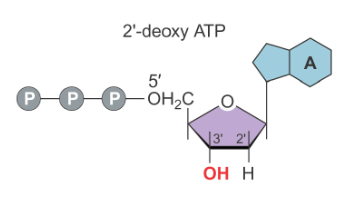
\includegraphics[scale=0.5]{images/dntp.png}
    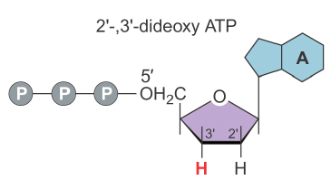
\includegraphics[scale=0.5]{images/ddntp.png}
    \caption{
        \emph{(Left)} normal dATP molecule, with an OH on the 3' end;
        \emph{(Right)} ddATP molecule, with just an H on the 3' end. These molecules can be labeled
        with radioactive phosphates or fluorophores for later detection.
    }
\end{figure}

We then let synthesis proceed as we do in a normal \emph{in vitro} DNA synthesis reaction. Note that
we actually run \emph{four} separate reactions, one for each type of ddNTP (ddATP, ddCTP, ddGTP,
ddTTP). When we let this synthesis run, at each base which requires a given dNTP, there is some
small probability of incorporating a ddNTP.\@

\begin{figure}[h!]
    \centering
    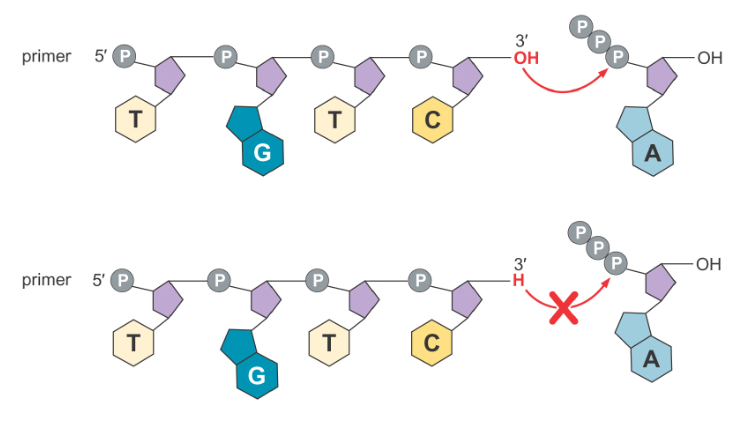
\includegraphics[scale=0.5]{images/synthesis.png}
    \caption{
        \emph{(Top)} The oxygen in the 3' OH can bond with the phosphate in the new dNTP instead of the hydrogen, thus joining
        the new dNTP into the chain;
        \emph{(Bottom)} If the last base incorporated is a ddNTP, the 3' end has just a hydrogen
        instead of an OH, and thus no new bases can be incorporated.
    }
\end{figure}

However, every time a ddNTP is incorporated, synthesis halts, because no new bases may be attached
to the 3' end of the resulting molecule. As a result, the synthesis will produce strands of varying
length, with a break at every point where the present ddNTP could be incorporated. Although it is
possible that a ddNTP is never incorporated at a given site, it is highly unlikely (statistically
speaking) because the reaction is being run with many strands of DNA at once, not just a single one.

\begin{figure}[h!]
    \centering
    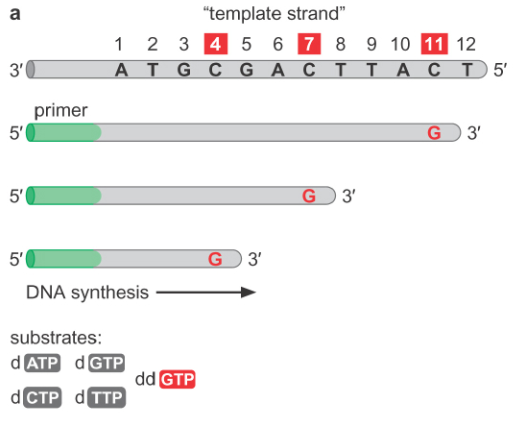
\includegraphics[scale=0.5]{images/stopped-synthesis.png}
    \caption{
        Synthesis will stop at different positions for different strands, but every G in the
        sequence will be represented by strands of the appropriate length.
   }
\end{figure}

Since we have strands of different lengths, we can use gel electrophoresis to visually separate the
strands. Note that we need to use a polyacrylamide gel instead of an agarose gel, because
polyacrylamide gels have a much greater resolution than agarose gel, and can be used to resolve the
length difference corresponding to a single base. When we put all of the four reactions we ran into
four lanes of the same gel, we can view all of the different sizes produced. In order to make sure
we get only the synthesized single strands and not the double stranded DNA, we run the gel under
denaturing conditions, which correspond to high temperatures and the addition of chemicals to
prevent hydrogen bonding.

\begin{figure}[h!]
    \centering
    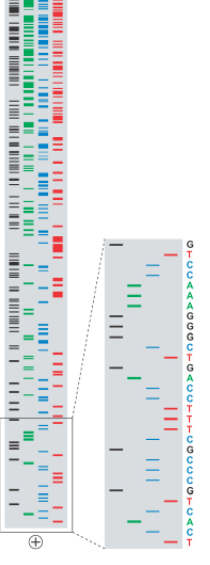
\includegraphics[scale=0.5,angle=-90]{images/lanes.png}
    \caption{
        Four lanes of gel electrophoresis, with a lane corresponding to each nucleotide type.
   }
\end{figure}

Finally, we can read off the sequence corresponding to the DNA by starting from the beginning of the
gel and looking at the dark bands in the gel. Each position should have exactly one band in the four
gels, which tells you which nucleotide is at that position. This method allows you to sequence long
fragments, with length mostly limited by the fact that larger strands require larger gels and it
becomes hard to distinguish different length sequences the larger the sequences are. 

There are a number of modern improvements to this method which make it practical. For instance,
instead of using four lanes of an electrophoresis gel and a radioactive phosphate marker, a single
capillary tube is used with fluorescent markers of different wavelengths for each nucleotide type. A
laser is placed over the capillary tube which measures the color under it at any given instant.
Then, the dimension of interest is no longer length of the gel but instead time, producing a series
of peaks for every wavelength.

\begin{figure}[h!]
    \centering
    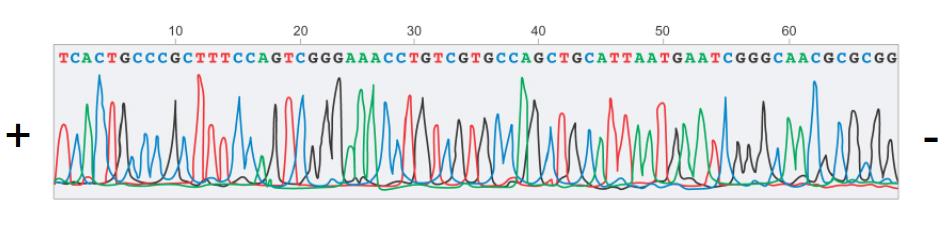
\includegraphics[scale=0.5]{images/peaks.png}
    \caption{
        Output from optical sensor measuring color of a location in the capillary tube. Peaks
        correspond to bases of a specific type.
   }
\end{figure}

Using signal processing techniques, we can detect the peaks in the signal seen above, and extract
the sequence of nucleotides, since each peak corresponds to a single nucleotide. Using current
techniques, Sanger sequencing can be made to work efficiently and cheaply, sequencing DNA pieces of
300--1000 base pairs.

\section*{Southern and Northern Blotting}

Southern and Northern blotting are techniques to visualize relative amounts of particular DNA or RNA
sequences in particular samples of each. The original inventor (after whom the technique was named),
Edwin Southern, performed this technique on DNA;\@ later, it was used on RNA as well, and was dubbed
Northern blotting when applied to RNA.\@ For the remainder of this explanation, I'll refer to the
sequences being targeted as DNA, which is the case for Southern blotting, but remember that Northern
blotting is simply the same thing with an RNA target sequence.

As usual, we begin by isolating the DNA (or RNA, in the Northern variant) that we wish to analyze.
We put this DNA onto some electrostatically interacting surface, such as nitrocellulose or nylon.
The DNA backbone binds (electrostatically) to the surface; note that the bases are still exposed for
hydrogen bonding when the DNA is bound. The sheet of nitrocellulose or nylon is then either heated
or exposed to ultraviolet light in order to permanently attach the DNA to its surface. At that
point, extra DNA is added in order to cover any parts of the sheet that were not covered by the
original DNA.\@ This prevents the probe from binding to the sheet itself. Also, chemicals are added to
reduce non-specific binding of the probe. Finally, a probe (usually RNA) is added. This probe has
radioactivally marked elements or fluorophores attached to it, so that when it binds to its
complementary DNA, it is visible. After hybridization of the probe, excess probe is washed away, and
the sheet is imaged.

\begin{figure}[h!]
    \centering
    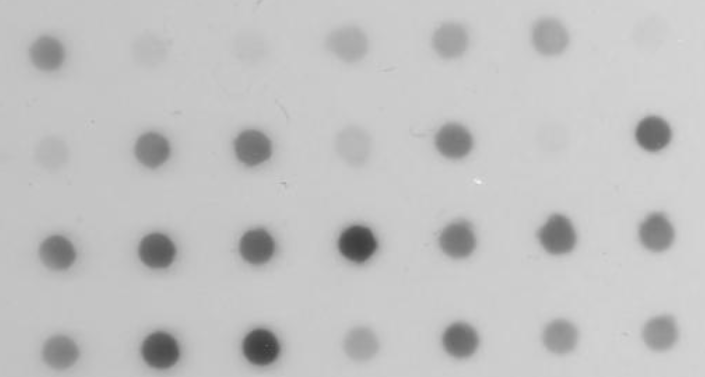
\includegraphics[scale=0.3]{images/blotting.png}
    \caption{
        (http://rsbweb.nih.gov/ij/docs/examples/dot-blot) The result of blotting can be a dot blot.
    }
\end{figure}

The result is an image which has varying brightness --- dark regions correspond to high concentrations
of the probe, while light regions correspond to low or nonexistent concentrations of the probe.
Since the probe is designed to bind to a very specific DNA sequence, this allows us to measure the
relative concentrations of DNA sequences in different samples.

In addition to using hand picked samples (as in a dot blot), we can combine gel electrophoresis with
blotting in order to measure relative concentrations of DNA sequences at the same time as measuring
the lengths of those sequences. 

\begin{figure}[h!]
    \centering
    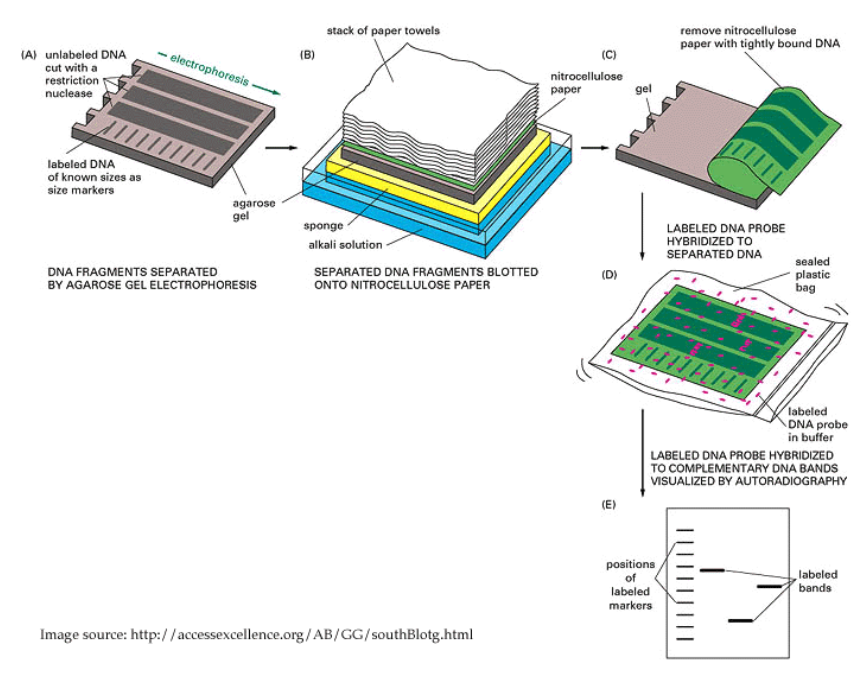
\includegraphics[scale=0.5]{images/gel-blotting-procedure.png}
    \caption{
        Procedure for blotting after a gel electrophoresis reaction.
    }
\end{figure}

In this case, the gel electrophoresis reaction is run, and the membrane is placed between the gel
and a stack of paper towels. The capillary action due to the paper towels pulls the DNA solution
upwards, and the DNA gets deposited onto the membrane in the location right above where it was in
the gel.

\begin{figure}[h!]
    \centering
    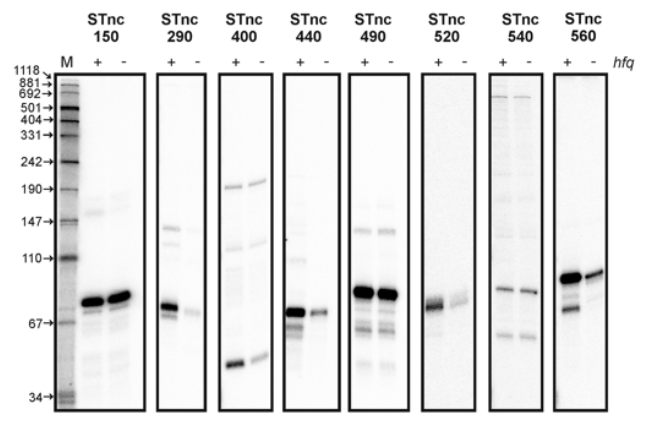
\includegraphics[scale=0.25]{images/gel-blotting-result.png}
    \caption{
        doi:10.1371/journal.pgen.1000163.g006
    }
\end{figure}

We get a result like what you see above --- namely, dark bands corresponding to high concentrations,
and bands further along indicating shorter sequences.

\section*{PCR}

\begin{figure}[h!]
    \begin{center}
        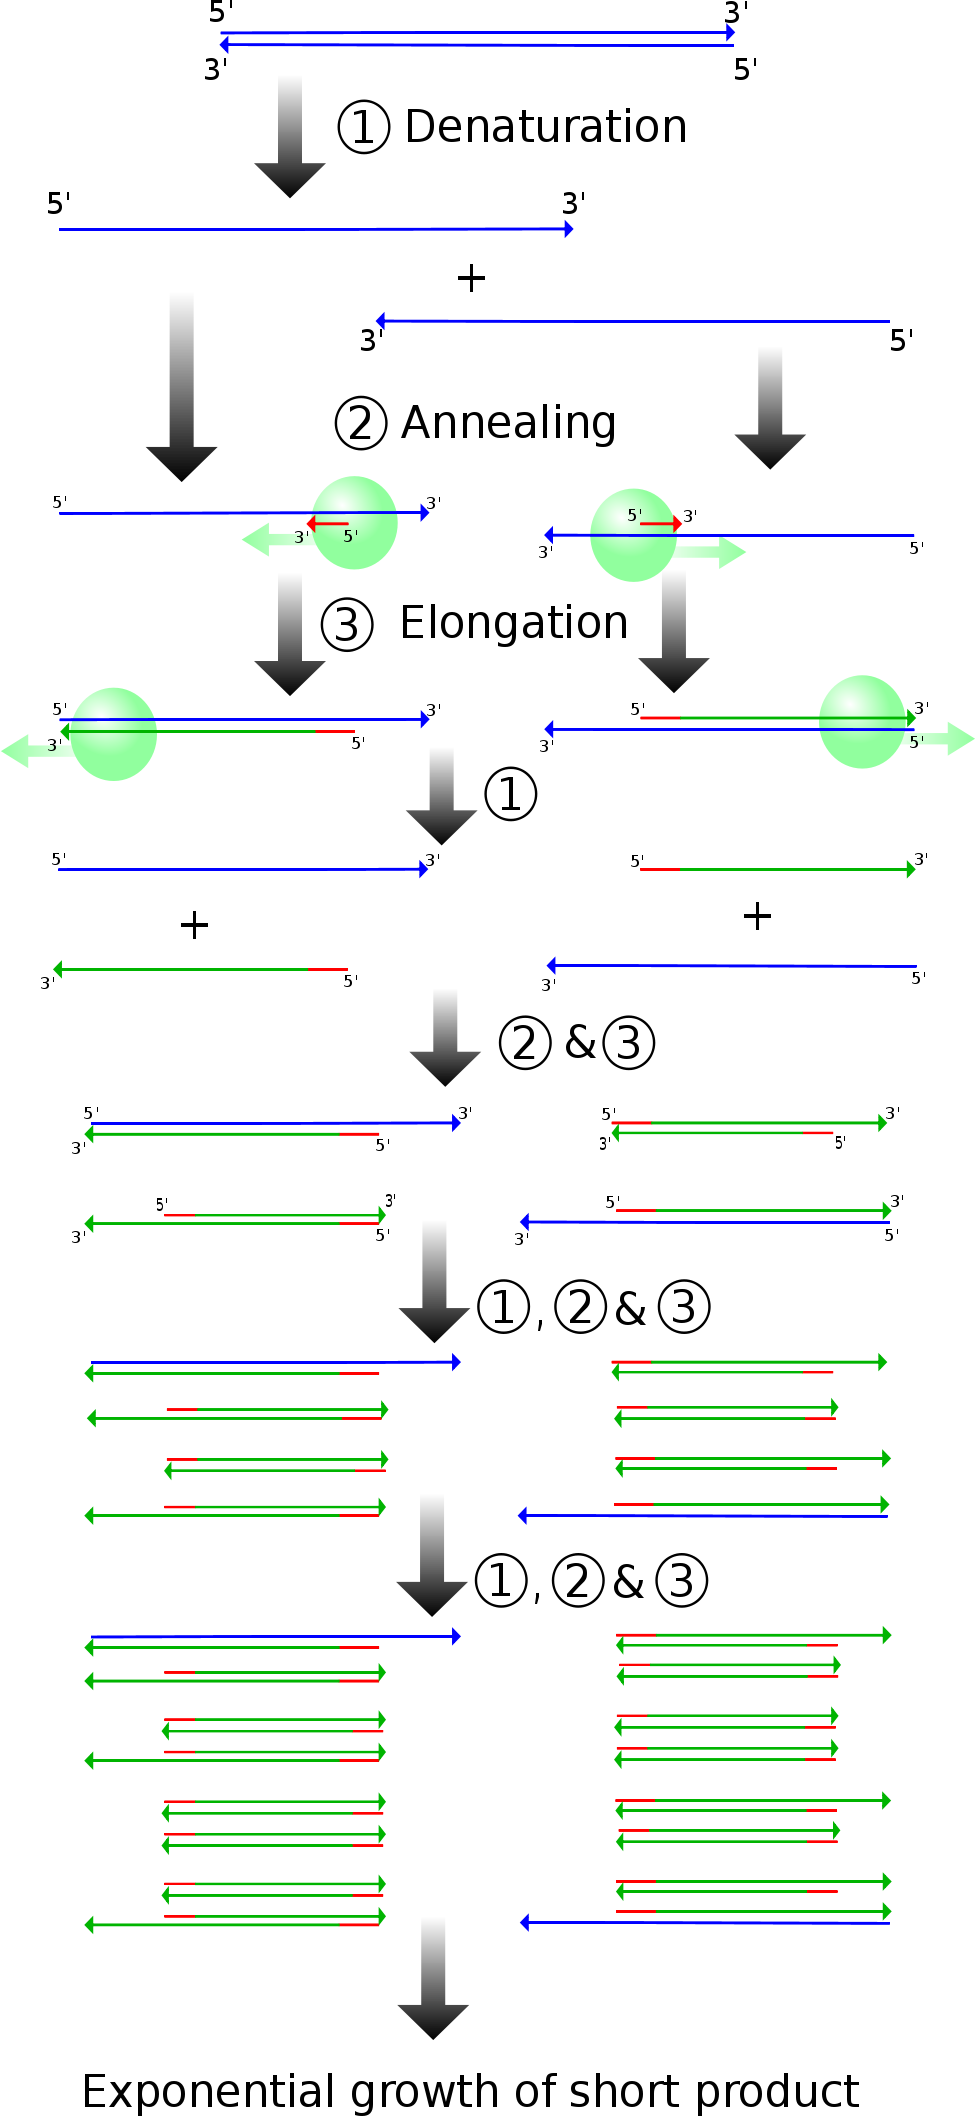
\includegraphics[width=0.5\textwidth]{images/pcr.png}
    \end{center}
    \caption{
        Diagram of PCR products and stages. \\\small (Madeleine Price Ball, Creative Commons License,
        sourced from http://en.wikipedia.org/wiki/File:PCR.svg)
    }
\end{figure}

Polymerase Chain Reaction (PCR) is a very common technique used to amplify specific sequences of
DNA.\@ This can be useful for sequencing, cloning, and other techniques that require high
concentrations of DNA.\@ \\

PCR is run in a solution with DNA containing the target sequence you wish to amplify, primers, and
DNA polymerase. First, the solution is heated to near boiling (94$^\circ$-96$^\circ$ C), so that the
DNA denatures and becomes single stranded. Once the DNA is single stranded, primers can bind to this
DNA.\@\\

The primers are designed to bracket the target sequence. The primers must be complementary to the 3'
end of both the template and coding sequences. After the DNA denatures, the temperature is lowered
to allow the primers to anneal to the DNA strands. Once the primers are bound, the temperature is
raised once more to the optimal temperature of the polymerase being used. A common polymerase is
known as \emph{Taq Polymerase}, and has an optimal temperature of approximately 75$^\circ$ C. The
polymerase binds to the primers and synthesizes complementary DNA until it reaches the end of the
strands. \\

Note that in the very first cycle, this creates long pieces of DNA that go ``indefinitely'' off to
one side of the target sequence. However, in future iterations, the primers bind such that the RNA
polymerase synthesizes towards the short end of the strand. Thus, \emph{only} the target sequence
gets amplified exponentially. Due to this exponential amplification, PCR is very sensitive, and can
be used to amplify sequences with very low initial concentrations. At 100\% efficiency (which is not
entirely realistic), the concentration of target sequence would double every iteration, and there
are usually somewhere between twenty and thirty iterations of PCR.\@

\clearpage
\section*{Quantitative PCR (qPCR)}

Quantitative PCR (qPCR) is an application of PCR in which instead of amplifying the target sequence,
you instead wish to measure the concentration or relative concentration of the target sequence in
the initial sample. 

PCR begins and proceeds as in a usual reaction. However, the concentration of the target sequence is
measured after every iteration of PCR.\@ One common way to do this is to have a double-stranded DNA
binding fluorophore; thus, when the DNA is allowed to cool and return to its double-stranded shape,
the dye binds to it and exhibits fluorescence. The more DNA is present, the more dye binds and thus
the greater the fluorescence. This allows us to measure and quantify the levels of DNA present after
each iteration.

\begin{figure}[h!]
    \centering
    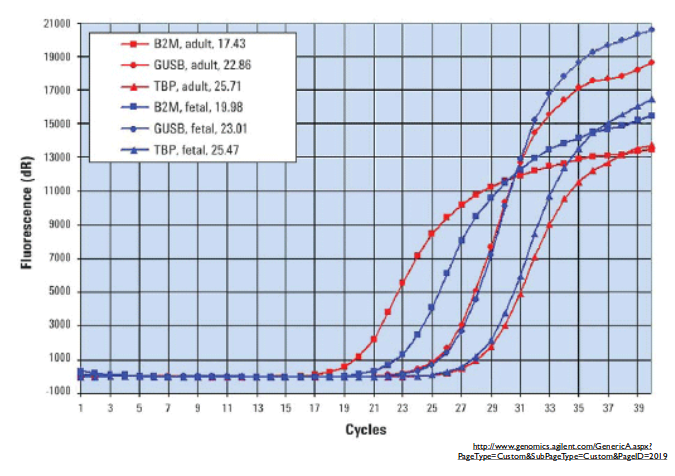
\includegraphics[scale=0.5]{images/qpcr.png}
    \caption{
        qPCR DNA concentration plotted against cycle number for several genes.
    }
\end{figure}

We get concentration plots that look like the plot above. Initially, the reaction runs
exponentially, with no limiting conditions. At the end of the reaction, however, it begins to run
out of primer or nucleotide components, and thus slows down until eventually it reaches a steady
state after which there is no more amplification. Together, these form what is essentially a
logistic curve.

In order to extract information from this, we can do one of two things. First of all, we can fit a
logistic curve to our data and use that to extrapolate to the start of the reaction in order to
determine the relative initial concentrations of the target sequences. We can also just measure the
vertical delta after a given number of cycles (close to the beginning of the amplification, while it
is still exponential, and not towards the end), and compare those values to determine which has
higher amplification. (In the figure above, for instance, what is reported just corresponds to
amplification after a given number of cycles.)

\clearpage
\section*{Reverse Transcription}

\begin{figure}[h!]
    \begin{center}
        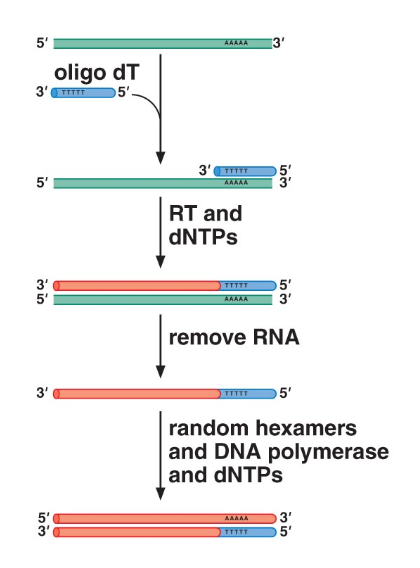
\includegraphics[width=0.5\textwidth]{images/reverse-transcription.png}
    \end{center}
    \caption{
        An RNA strand being reverse transcribed into DNA.\@
    }
\end{figure}

Reverse transcription is a process by which we can convert strands of RNA back into DNA.\@ The
generated DNA is known as complementary DNA (cDNA), and is created by enzymes known as reverse
transcriptases. \\

The process is initiated with an oligo (which acts as a primer), reverse transcriptase, and
nucleotides (dNTPs). The transcriptase synthesizes a complementary DNA strand to the given RNA
sequences. Then, the RNA is removed, leaving a DNA strand with the RNA primer at the beginning.
Afterwards, DNA polymerase synthesizes a strand complementary to that one  \emph{entirely} out of
DNA, yielding a copy of the original RNA as a DNA strand.\\

Note that due to the complexity of this process (multiply involved polymerases, etc), it turns out
to be incredibly error prone and causes a rather high mutation rate. Retroviruses, for example, have
a genome that consists entirely of RNA, and use reverse transcription to reproduce; this results in
a very high mutation rate among them.

\section*{DNASel Footprinting}

In class, we discussed the \emph{lac} operon, and how the repressor binds to a region next to the
DNA that the RNA polymerase covers. 

\begin{figure}[h!]
    \centering
    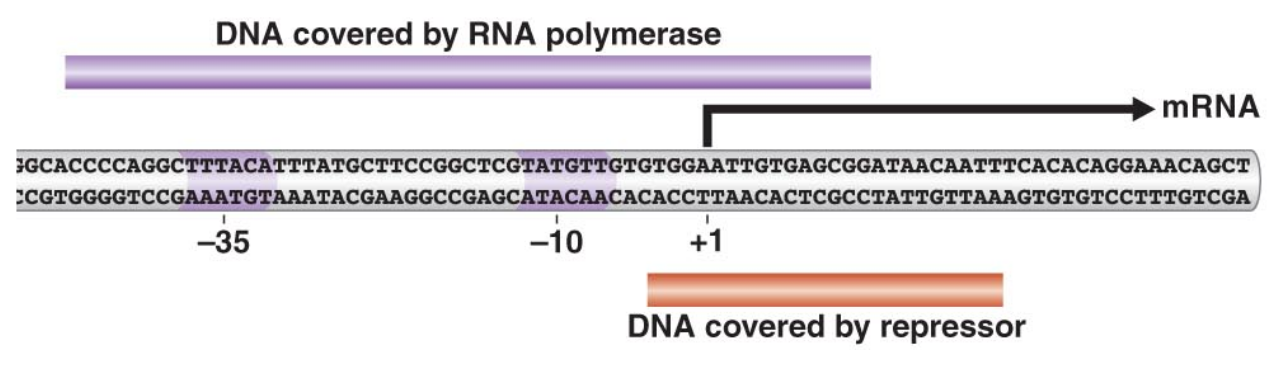
\includegraphics[scale=0.2]{images/lac-repressor.png}
\end{figure}

We saw the figure above, which depicts the regions of the DNA that each of the proteins covers when
bound to the DNA.\@ This figure leads to a natural question --- namely, how can we determine the data
presented?

\begin{figure}[h!]
    \begin{center}
        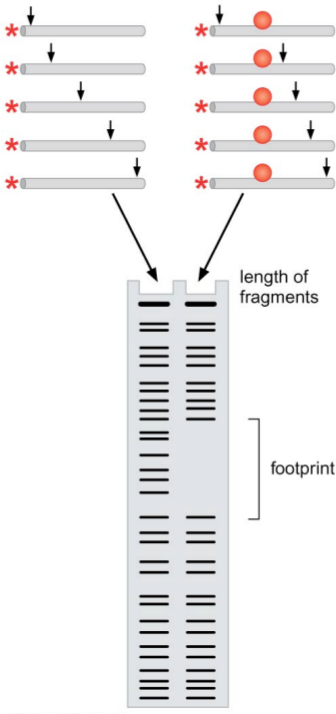
\includegraphics[width=0.3\textwidth]{images/dnasel-footprinting.png}
    \end{center}
    \caption{
        Diagram of DNAsel footprinting. On the left you can see the DNA alone treated with the endonuclease, while
        the right column corresponds to DNA with a bound protein being treated with the
        endonuclease.
    }
\end{figure}

DNAsel footprinting is a technique for determining which bases a protein covers when it binds to the
DNA.\@ Note that this does \emph{not} just determine the points of contact of the protein to the DNA,
but instead determines which bases are covered (and thus prevented from binding to other proteins). 

DNAsel footprinting is an in vitro technique. Begin by taking some DNA of interest (such as the
\emph{lac} promoter and the region around it) and radioactively labeling the 5' end of the DNA (with
$^{32}$P). Next, treat the DNA with DNAse1. DNAse1 is an endonuclease. While exonucleases is
something which cleaves nucleotides from the end of a polynucleotide, an endonuclease cleaves
polynucleotides starting at some position in the middle and going from 5' to 3'. DNAse1 is an
endonuclease which has no affinity for a particular DNA sequence, so it effectively cleaves the DNA
at a random position.

Once the DNA has been treated with the endonuclease, use an acrylamide gel to visualize the
radioactively labeled sequences. Since we only labeled the 5' ends of the sequences, only the
lengths of the 5' ends of the DNA fragments will be visualized. Note that we calibrate the amount of
DNAse to the concentration of DNA, in order to prevent the same DNA from being cleaved multiple
times.

In addition to doing this reaction with the DNA of interest, we also do it with the same DNA in the
presence of the protein of interest. The protein will bind to the DNA, and cover some of the bases.
Then, when the DNAse attempts to bind to the DNA at those bases in order to cleave the DNA, it will
be unable to bind. Thus, there will be a gap in the fragment lengths --- a footprint --- in the
locations where the endonuclease was unable to bind. If we run a simultaneous Sanger sequencing
reaction, we will know exactly where that gap was and what bases it corresponds to, and this will
tell us which bases the protein covers.

Note that this procedure isn't completely precise. For instance, the endonuclease itself takes up
some number of bases, so there may be a part of the DNA strand that is never cleaved but is also
uncovered by the protein we're interested in --- it is simply close to the covered bases. This makes
DNAsel footprinting slightly overestimate the size of the covered region, but usually by no more
than (approximately) ten nucleotides.

\section*{Yeast two-hybrid assay}
In class, we discussed the following figure, in which we can see RNA polymerase binding to a
promoter as well as the $\alpha$-CTD subunit binding to the activator CRP.\@

\begin{figure}[h!]
    \centering
    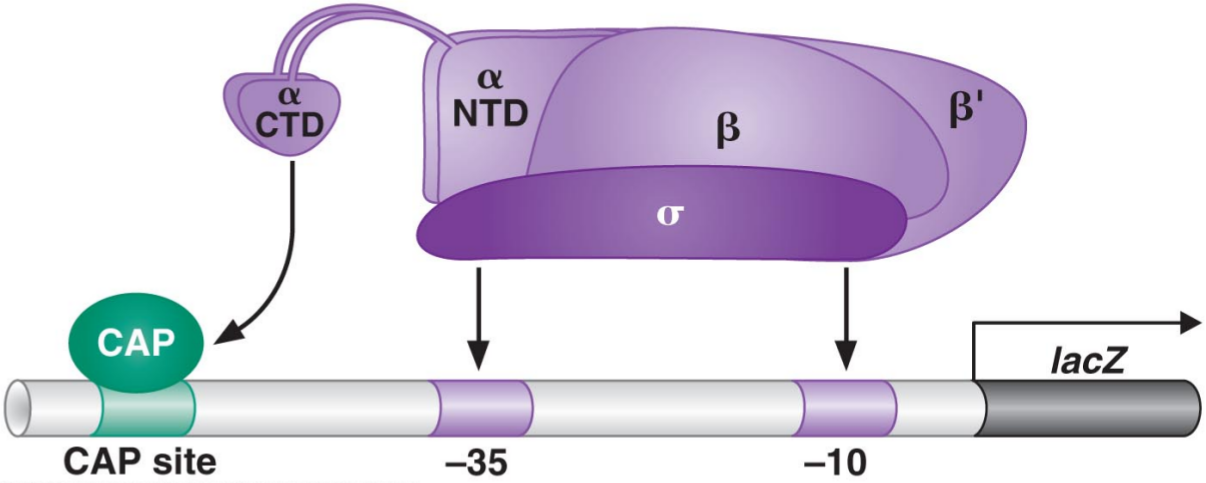
\includegraphics[width=0.6\textwidth]{images/cap-rnap.png}
    \caption{
        $\alpha$ C-terminus domain of RNA polymerase interacts with CRP, which serves as an
        activator.
    }
\end{figure}

This led to a natural question: suppose that we didn't know about CRP but instead wanted to find
\emph{all} proteins that bound to a given target protein. How could we do this?

The yeast two-hybrid assay is an approach to doing this. It relies on the fact that activators, such
as the \emph{Gal4} activator (which binds to a \emph{Gal4} binding site and is involved in galactose
metabolism in yeast), are composed of two functionally separate pieces. One of them contains the
DNA-binding domain (which has the function of chemically bonding with the DNA in the binding site),
while the other contains the activating region, which is responsible for binding to the RNA
polymerase in order to increase its affinity and thus activate transcription.

\begin{figure}[h!]
    \begin{center}
        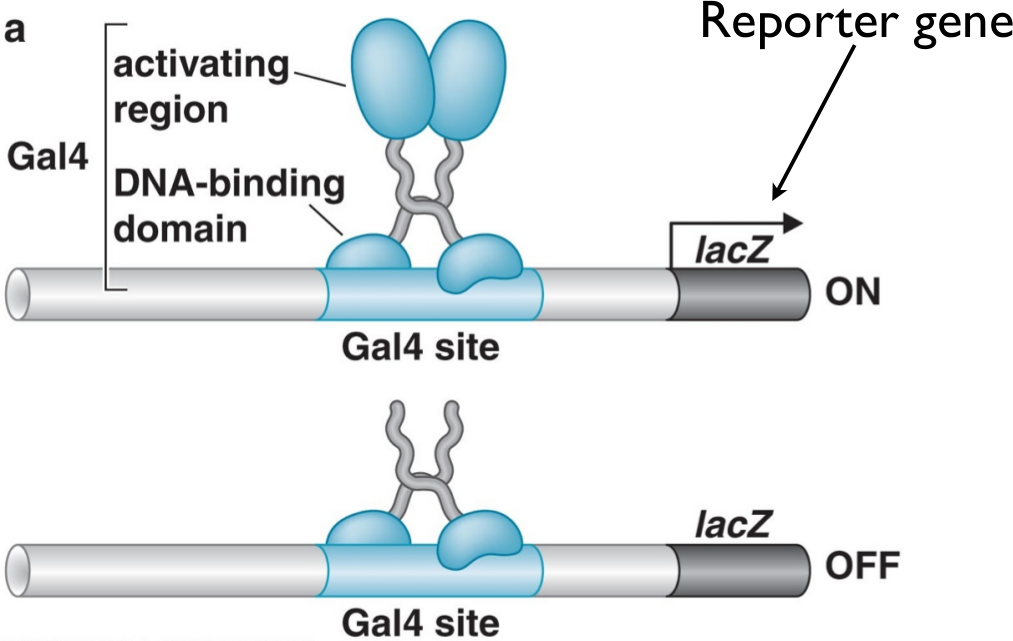
\includegraphics[width=0.6\textwidth]{images/gal4.png}
    \end{center}
    \caption{
        \emph{Gal4} protein contains an activation region and a DNA binding domain. The coding
        sequence for the activation region can be cleaved from the sequence for the DNA binding
        domain.
    }
\end{figure}

The key insight is that we can \emph{separate} these two regions in the DNA itself. Using
restriction enzymes and ligation techniques we've discussed previously, we can separate the DNA
binding domain and the activating region into two separate plasmids. Then, we can fuse our protein
of interest (via these same techniques) into the DNA binding domain. The resulting complex can be
referred to as the \emph{bait}, because it will bind only to proteins that interact with our target
protein.

We then generate a very large library of proteins which are attached to the activation domain
sequence. In fact, each plasmid we generate may have a separate protein sequence attached to the
activation domain. Once we have bait and prey plasmids, we can force yeast to incorporate these
plasmids.

Suppose that a yeast cell incorporates the bait plasmid and a prey plasmid which happens to have the
sequence for the activation domain bound to a sequence for some protein that the protein of interest
interacts with. Then, when the bait and prey are translated, the DNA binding domain (attached to the
bait) will bind to the DNA next to the \emph{LacZ} promoter, while the prey will interact with the
bait, thus bringing the activator domain in proximity to the \emph{LacZ} promoter. As a result of
this interaction, the \emph{LacZ} gene will be activated and highly expressed in the cell.

Suppose, instead, that a yeast cell incorporates a prey plasmid which has a protein coding sequence
for a protein that does \emph{not} interact with the bait. In that case, the activation domain will
never be brought close to the promoter, and thus the \emph{LacZ} gene will not be expressed nearly
as strongly as it is in the other case. Thus, expression of \emph{LacZ} is tightly coupled with
whether a yeast cell incorporated a prey plasmid for a protein that interacts with the target
protein.


\begin{figure}[h!]
    \begin{center}
        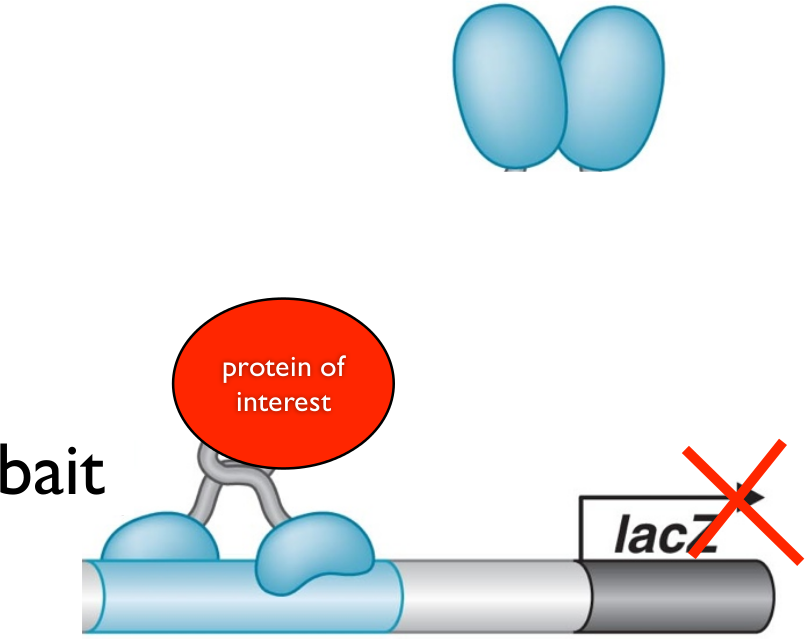
\includegraphics[width=0.40\textwidth]{images/bait.png}\\
        \vspace*{2em}
        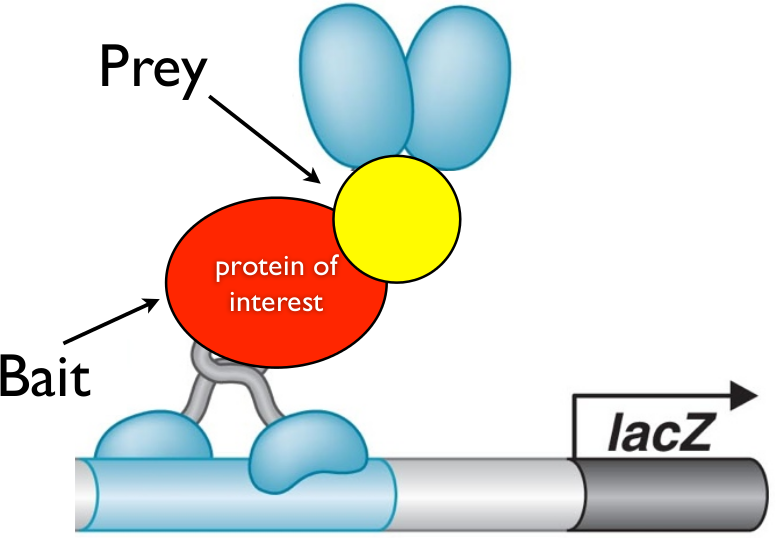
\includegraphics[width=0.40\textwidth]{images/bait-and-prey.png}
    \end{center}
    \caption{
        \emph{(Top)} Protein of interest attached to DNA binding sequence of activator protein.
        Without appropriate prey, no activation occurs.\\
        \emph{(Bottom)} When prey protein interacts with bait, activation domain is proximal to the
        promoter, and thus transcription is activated.
    }
\end{figure}

Yeast cells on a plate will form distinct colonies, each of which is descended from a single cell,
so each colony will have the same plasmids that the mother yeast cell contained. We can then use
\emph{X-gal} to test for the expression of \emph{LacZ}. When the \emph{LacZ} gene is expressed, it
creates mRNA which codes for a protein known as $\beta$-galactosidase. $\beta$-galactosidase cleaves
\emph{X-gal} (which is composed of a particular molecule bound to a galactose) into the constituent
parts; while \emph{X-gal} itself is colorless, the \emph{X} molecule alone (without the galactose)
is visibly blue. Thus, in the presence of \emph{X-gal}, the yeast cells which have prey that
interacts with the bait and thus have strong expression of \emph{LacZ} will be visibly blue, while
the others will be colorless.

We can use the color of yeast colonies to separate out the colonies which received prey plasmids
that interact with the bait. We can purify out the prey plasmids from these blue yeast colonies and
sequence them, yielding the sequence of a protein that interacts with our target protein (which was
attached to the bait protein).

Although this technique can be very useful, it has a number of problems as a result of which it is a
much better hypothesis \emph{generating} tool (as opposed to one which can be used to check a
hypothesis). This technique can easily fail to find proteins that interact with our target protein,
because it may be that the proteins need to be modified post transcriptionally (which may not happen
when they are bound to the activation domain) or perhaps they must be localized to a particular part
of the cell. Similarly, the technique can find proteins that do not actually interact with the
target protein --- for instance, if the target protein is only expressed in high temperature
environments, the library may include a protein that seems to interact with the target protein but
actually has no biological relevance, because it is only expressed in low temperature environments
(and thus the interaction can never actually happen). The technique may fail to find proteins simply
because, due to the complexities of protein folding and interactions, glueing together the sequences
of two proteins will \emph{not} necessarily yield a protein with the same interactions as the
separate proteins.

\section*{Western Blotting}

In previous technique primers, we discussed Northern and Southern blotting, which are techniques
used to visualize the abundance and potentially sizes of RNA and DNA, respectively. A similar
technique exists for proteins and is appropriately named \emph{Western blotting}, or occasionally
Western hybridization.

The fundamental difference between Western blotting and Northern and Southern blotting is the probe.
While RNA and DNA can both use a similar RNA probe, we cannot use an RNA probe to visualize
proteins. Instead, we must use antibodies. 

Antibodies are large Y-shaped proteins produced by immune systems to identify and destroy foreign
cells and viruses. For the purposes of Western blotting, the protein we're interested in targeting
may be introduced to a cell culture or a mammal (such as a mouse) in order to induce an immune
response. The immune system will produce an antibody (known as the primary antibody) which binds to
the target protein. We can purify this antibody from the cells and then use it as a probe.

Once we have an antibody probe, the process of a Western blot is very similar to that of a Northern
or Southern blot. We run our proteins through a gel, which separates the proteins based on their
size; we transfer these proteins to a membrane; we block any unused area on the membrane to prevent
antibodies from binding there by placing the membrane in a solution of non-specifically binding
protein; finally, we visualize the results by letting the labeled probe antibody bind to the target
proteins. 

Note that although it is possible to label the primary antibodies (those created by the immune
system response) with fluorescent molecules and then visualize them, this can be rather expensive,
as each antibody must be custom. However, instead, we can use a fluorophore-labeled secondary
antibody. Secondary antibodies are antibodies which bind to the primary antibodies; however, unlike
primary antibodies, secondary antibodies will bind to almost \emph{any} primary antibody, and are
thus nonspecific and much cheaper.

\section*{Chromatin immunoprecipitation (ChIP)}

\begin{figure}[h!]
    \begin{center}
        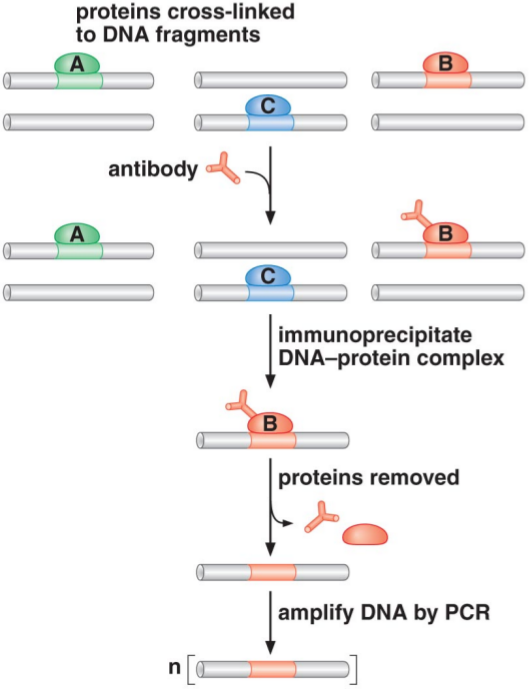
\includegraphics[width=0.6\textwidth]{images/chip.png}
    \end{center}
    \caption{
        Chromatin Immunoprecipitation.
    }
\end{figure}

While the yeast two-hybrid assay can be used to detect all \emph{proteins} that interact with a
particular protein, we may also be interested in detecting all DNA locations which a given protein
interacts with. We can use chromatin immunoprecipitation, a technique which precipitates out DNA
sequences which interact with a protein, in order to detect these DNA locations.

When doing chromatin immunoprecipitation, cells are first fixed with a cross-linking agent, such as
formaldehyde or ultraviolet light. Cross-linking is a reaction in which a protein can be covalently
bound to DNA.\@ At this stage, all proteins may be bound to DNA in various places, as we can see in
the first row in the image to the right. We then shear DNA, which breaks it into fragments only
several hundred bases in length. (If we did not shear the DNA, we would end up precipitating the
entire chromosome, instead of only the regions which had proteins bound to them.)

Next, we mix this solution with antibodies specific to the protein we wish to target. These
antibodies are created in a manner similar to the one we used for Western blots. The antibodies bind
to the protein we are interested in (which is still cross-linked to the DNA regions it interacts
with). We can then couple these antibodies with another molecule, such as agarose or magnetic beads.
These molecules form the immunoprecipitate, which allow us to precipitate out or otherwise separate
the antibodies and everything they're bound from the rest of the solution.

Once we have separated these out, we remove all the bound proteins. (This is why we require that the
cross-linking be reversible.) Once we remove the proteins, we are left with only DNA.\@ We can then
amplify this DNA through a polymerase chain reaction (PCR). Sequencing this DNA will give only the
fragments which contain the DNA sequences which the target protein binds to, thus identifying those
sequences.

\section*{Electrophoretic mobility shift assay (EMSA/gel shift)}


\begin{figure}[h!]
    \begin{center}
        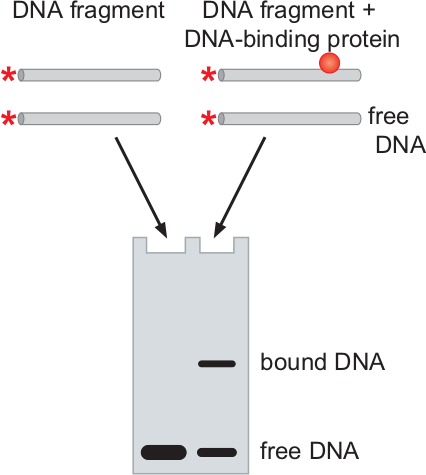
\includegraphics[width=0.5\textwidth]{images/emsa.png}
    \end{center}
    \caption{
        Electrophoresis mobility shift assay.
    }
\end{figure}

In addition to locating which DNA a protein interacts with, as we can do with chromatin
immunoprecipitation, we may want to determine whether a protein interacts with a piece of DNA, or
the order in which several proteins interact with a DNA binding site. This type of experiment may be
done via an electrophoretic mobility shift assay (EMSA), commonly known as a gel or band shift
assay, and can be very useful for studying processes such as transcription (especially initiation)
and DNA replication.

The fundamental fact that EMSA relies upon is that DNA strands that have proteins bound to them will
move slower in an electrophoresis gel than DNA strands with no proteins bound to them, and that
larger bound proteins will result in a slower movement (lower electrophoretic mobility) than smaller
bound proteins. 

We begin by taking a single or double stranded piece of DNA containing the binding site of interest
and labeling it radioactively. Although we can label it with a fluorophore, this may be harder,
because the fluorophore must be placed such that it does not interfere with the binding of proteins
to the DNA.\@ This labeled piece of DNA is sometimes referred to as the ``probe''. 

Next, we mix our probe with the protein (or proteins) of interest. We let them interact and then
separate out the molecules of different electrophoretic mobilities in a \emph{non}denaturing gel.
Note that unlike other techniques we've discussed, the gel must \emph{not} denature the molecules,
as that would cause them to unbind and render the entire technique pointless. In another lane of the
same gel, we can run the DNA probe without the proteins. We can then image the gel and observe the
bands in both gels; if the protein binds to the DNA, then we will note a significant shift in the
band. The diagram on the left, for instance, depicts a single protein binding to the DNA;\@ you can
see that some of the DNA was bound, producing a band closer to the start location (since it moved
slower), while some of the DNA remained free, thus creating a band in the same place as the unbound
DNA on the DNA-only lane.

Note that we can use EMSA to study the interactions of multiple proteins as well. These interactions
can be due to multiple binding sites, or even due to subsequent proteins interacting with proteins
that have bound to the DNA.\@ As each additional protein binds, it will reduce the mobility, thus
causing a greater shift. This can help identify how a series of proteins interacts with a strand of
DNA --- since larger proteins will slow the DNA down more than smaller once, you can distinguish
which protein bound to the DNA.\@ (When you have two identically sized proteins, you can differentiate
between them by adding an antibody that targets only one of them; the antibody will bind to that
protein, effectively increasing its size and allowing you to differentiate from the other one. This
technique is known as a \emph{supershift assay}.)

One weakness of this technique is that while it can confirm binding of protein to DNA, it cannot
identify the precise binding site in the DNA strand. However, other techniques may be used to
rectify this. For instance, mutations may be introduced into the DNA strand to assess the
specificity of the protein binding. Another common technique is to run extra lanes with different
oligonucleotides which compete with the DNA strand for binding; if you use oligonucleotides of known
sequence, you can identify the sequence of the binding site in the DNA.\@

\end{document}
